% =====================================================
% Face-Preserved Hybrid Framework for Lightweight 
% Photo-to-Anime Translation on Resource-Constrained Devices
% IEEE Journal/Conference Paper
% =====================================================
\documentclass[journal]{IEEEtran}

% --- Packages ---
\usepackage{cite}
\usepackage{amsmath,amssymb,amsfonts}
\usepackage{algorithmic}
\usepackage{algorithm}
\usepackage{graphicx}
\usepackage{textcomp}
\usepackage{xcolor}
\usepackage{booktabs}
\usepackage{multirow}
\usepackage{url}
\usepackage{hyperref}
\usepackage{tabularx}
\usepackage{balance}

% --- Graphics path ---
\graphicspath{{figures/}{../figChap1/}{../figChap2/}{../figChap3/}}

% --- Custom commands ---
\newcommand{\ie}{\textit{i.e.}}
\newcommand{\eg}{\textit{e.g.}}
\newcommand{\etal}{\textit{et al.}}
\newcommand{\wrt}{\textit{w.r.t.}}

\begin{document}

% =====================================================
% TITLE
% =====================================================
\title{Face-Preserved Hybrid Framework for Lightweight Photo-to-Anime Translation on Resource-Constrained Devices}

\author{
\IEEEauthorblockN{Nhan Trong Nguyen\IEEEauthorrefmark{1} and Chau Thi Ma\IEEEauthorrefmark{2}}
\IEEEauthorblockA{
Faculty of Information Technology\\
University of Engineering and Technology\\
Vietnam National University, Hanoi\\
Email: \IEEEauthorrefmark{1}24025149@vnu.edu.vn,
\IEEEauthorrefmark{2}chaumt@vnu.edu.vn}
}

\maketitle
`'
% =====================================================
% ABSTRACT
% =====================================================
\begin{abstract}
Recent advances in generative adversarial networks (GANs) have enabled automatic photo-to-anime translation, yet existing approaches struggle to simultaneously preserve facial identity and maintain real-time inference on resource-constrained devices. Meanwhile, diffusion-based methods achieve impressive visual quality but demand gigabytes of model storage and seconds per image, rendering them impractical for edge deployment. In this paper, we propose a \textit{Face-Preserved Hybrid Framework} that integrates a lightweight Double-Tail GAN (DTGAN) backbone with an automated face detection and enhancement pipeline. Our framework operates in three adaptive modes---Face, Landscape, and Hybrid---with graceful degradation when no face is detected. Two key engineering design choices drive quality: (1)~a \textit{Symmetric Margin Expansion} procedure that pads face bounding boxes with a 50\% margin, enforces a 1:1 aspect ratio, and clamps to image boundaries---preserving critical facial context (hair, ears, neck) for the generator; and (2)~\textit{Feathered Blending} via Gaussian-smoothed alpha compositing that eliminates visible seams when merging high-resolution face crops onto landscape-processed backgrounds. Our system achieves a Fr\'{e}chet Inception Distance (FID) of 58.6 and LPIPS of 0.384 in Face Mode, while requiring only 9.1\,MB of model storage and running at 42\,FPS---over 20$\times$ faster and 200$\times$ smaller than comparable diffusion-based solutions. A structured user study with 42 participants confirms statistically significant improvements in identity preservation and visual quality over baseline methods.
\end{abstract}

\begin{IEEEkeywords}
Generative adversarial networks, anime style transfer, face detection, image compositing, edge AI, lightweight deployment, ONNX Runtime
\end{IEEEkeywords}

% =====================================================
% I. INTRODUCTION
% =====================================================
\section{Introduction}
\label{sec:intro}

The global anime market has grown to an estimated \$81.96 billion in 2024 and is projected to exceed \$200 billion by 2034, fueling unprecedented demand for automated content creation tools that can bridge the gap between photographic imagery and the distinctive aesthetic of Japanese animation. Photo-to-anime translation---the task of transforming a real photograph into an anime-style rendition while preserving semantic content---belongs to the broader class of unpaired image-to-image translation problems~\cite{Zhu2017, Isola2017}. Unlike traditional neural style transfer~\cite{Johnson2016}, which often produces texture artifacts when source and target domains differ substantially, GAN-based approaches learn domain-specific transformations that capture the flat color regions, sharp outlines, and simplified textures characteristic of anime art~\cite{Chen2018CartoonGAN, Chen2020, Liu2024}.

Despite significant progress, two fundamental challenges remain underexplored. First, most existing GAN-based anime stylization methods---including CycleGAN~\cite{Zhu2017}, CartoonGAN~\cite{Chen2018CartoonGAN}, and AnimeGANv2~\cite{ChenLiu2020}---process the entire image at a uniform resolution. When a portrait photograph contains faces that occupy a small fraction of the frame, facial details such as eyes, nose, and lip contours are lost during the style transfer process, severely degrading identity preservation. Second, the recent emergence of diffusion models~\cite{Ho2020, Rombach2022} has shifted the generative modeling landscape. Systems such as Stable Diffusion combined with ControlNet~\cite{Zhang2023ControlNet} can produce remarkable anime-style outputs, yet they demand 2--7\,GB of model storage, 8--16\,GB of GPU memory, and achieve only 0.5--2\,FPS---making them entirely impractical for mobile applications, web services with concurrent users, or embedded systems.

This paper proposes a \textit{Face-Preserved Hybrid Framework} for lightweight photo-to-anime translation that explicitly addresses both challenges. Built upon the AnimeGANv3 Double-Tail GAN (DTGAN)~\cite{Liu2024} as a pretrained backbone, our framework introduces an automated face detection, extraction, and enhancement pipeline that adaptively coordinates global landscape stylization with high-resolution local face synthesis. The system operates in three modes---Face Mode (portrait-optimized), Landscape Mode (full-image), and Hybrid Mode (combined)---with an automatic graceful degradation mechanism.

The main contributions of this paper are summarized as follows:
\begin{enumerate}
\item We propose an end-to-end hybrid framework for photo-to-anime translation that adaptively coordinates global landscape stylization and high-resolution local face synthesis within a unified pipeline, including a parallelized CPU-GPU training workflow for real-time loss computation.

\item We design a \textit{Symmetric Margin Expansion} procedure that pads, squares, and clamps detected face bounding boxes to include surrounding context (hair, ears, neck) needed for natural anime rendering. We empirically validate $m = 0.5$ as the optimal expansion ratio through ablation over FID and LPIPS.

\item We employ \textit{Feathered Blending}---Gaussian-smoothed alpha compositing---to seamlessly merge high-resolution face crops with landscape-processed backgrounds, avoiding the color bleeding introduced by Poisson editing while adding negligible latency ($<$5\,ms per face).

\item We conduct extensive quantitative evaluations (FID, LPIPS, FPS) and a structured user study with 42 participants, demonstrating statistically significant superiority of our hybrid approach in identity preservation and visual quality, with the complete system requiring only 9.1\,MB and running at 42\,FPS.
\end{enumerate}


% =====================================================
% II. RELATED WORK
% =====================================================
\section{Related Work}
\label{sec:related}

\subsection{GAN-Based Anime Style Transfer}

The foundational work of Goodfellow~\etal~\cite{Goodfellow2014} established GANs as a powerful framework for image synthesis. For unpaired image translation, CycleGAN~\cite{Zhu2017} introduced cycle consistency constraints that enable learning without paired training data, though it often produces color artifacts and struggles with fine facial details. CartoonGAN~\cite{Chen2018CartoonGAN} proposed edge-promoting adversarial loss specifically for cartoon stylization, while U-GAT-IT~\cite{Kim2020} incorporated attention modules and adaptive layer-instance normalization to improve translation quality.

The AnimeGAN series~\cite{Chen2020, ChenLiu2020, Liu2024} represents the most targeted line of research for anime-specific stylization. AnimeGANv3 (DTGAN)~\cite{Liu2024} introduces a Double-Tail Generator architecture with a shared encoder and two specialized decoders: a Support Tail that learns structural outlines and a Main Tail that refines color distributions. Combined with Layer-Adaptive Denormalization (LADE) and a multi-component loss system including region smoothing and fine-grained revision losses, DTGAN achieves state-of-the-art quality-efficiency tradeoffs with only $\sim$1.02M parameters. Our work builds upon DTGAN as a pretrained backbone and extends it with a face-aware hybrid processing pipeline.

StyleGAN-based approaches~\cite{Karras2019, Richardson2021} achieve exceptional quality through GAN inversion into the latent $\mathcal{W}$ space, but require tens of millions of parameters and hundreds of optimization steps per image, making them unsuitable for real-time deployment.

\subsection{Diffusion-Based Approaches}

Denoising diffusion probabilistic models (DDPMs)~\cite{Ho2020} have emerged as the dominant paradigm for image generation, with Dhariwal and Nichol~\cite{Dhariwal2021} demonstrating that diffusion models can surpass GANs on standard benchmarks. Latent Diffusion Models~\cite{Rombach2022} (underlying Stable Diffusion) reduce computational costs by operating in a compressed latent space, while ControlNet~\cite{Zhang2023ControlNet} enables geometric conditioning for structure-preserving style transfer. DiffusionCLIP~\cite{Kim2022DiffusionCLIP} combines diffusion models with CLIP for text-guided style manipulation.

However, these methods impose severe computational requirements: Stable Diffusion models occupy 2--7\,GB of storage and require 8--16\,GB of GPU memory for inference at 0.5--2\,FPS. This makes diffusion-based approaches fundamentally incompatible with resource-constrained deployment scenarios---the exact context targeted by our work.

\subsection{Face-Aware Image Processing}

Face detection has evolved from Viola-Jones cascades to modern single-shot detectors such as RetinaFace~\cite{Deng2019RetinaFace}, which simultaneously predicts bounding boxes, confidence scores, and five facial landmarks through multi-task learning on a Feature Pyramid Network~\cite{Lin2017FPN}. The MobileNet-0.25 variant~\cite{Howard2017MobileNet} provides an ultra-lightweight backbone ($\sim$500\,KB) suitable for edge deployment.

While face-aware processing has been explored in super-resolution and face restoration, its application to anime-style transfer remains largely unexplored. Our work is, to the best of our knowledge, the first to integrate face detection with margin expansion and feathered blending into a unified anime stylization pipeline.


% =====================================================
% III. PROPOSED METHOD
% =====================================================
\section{Proposed Method}
\label{sec:method}

\subsection{System Overview}
\label{subsec:overview}

Fig.~\ref{fig:pipeline} illustrates our Face-Preserved Hybrid Framework. Given an input photograph $I \in \mathbb{R}^{H \times W \times 3}$, the system executes the following stages: (1)~face detection via RetinaFace~\cite{Deng2019RetinaFace} to obtain bounding boxes $\{B_i\}_{i=1}^{N}$ and facial landmarks; (2)~mode selection based on detection results and user preference; (3)~stylization through the DTGAN backbone via ONNX Runtime~\cite{ONNX2019}; and (4)~compositing via Feathered Blending for Hybrid Mode.

The framework supports three operating modes:
\begin{itemize}
\item \textbf{Face Mode}: The largest detected face is extracted, expanded via Symmetric Margin Expansion, resized to $512 \times 512$, and processed through the generator. Best suited for portrait and avatar applications.
\item \textbf{Landscape Mode}: The full image is resized (dimensions divisible by 8) and processed directly. Optimal for scenery without prominent faces.
\item \textbf{Hybrid Mode}: The background is processed via Landscape Mode, while each detected face is independently processed via Face Mode at $512 \times 512$ and composited back using Feathered Blending. This mode combines high-quality facial details with anime-styled backgrounds.
\end{itemize}

A critical design principle is \textit{graceful degradation}: when Face or Hybrid Mode is selected but no face is detected (confidence below 0.8), the system automatically falls back to Landscape Mode, ensuring the pipeline never produces an error state.

\begin{figure}[t]
\centering
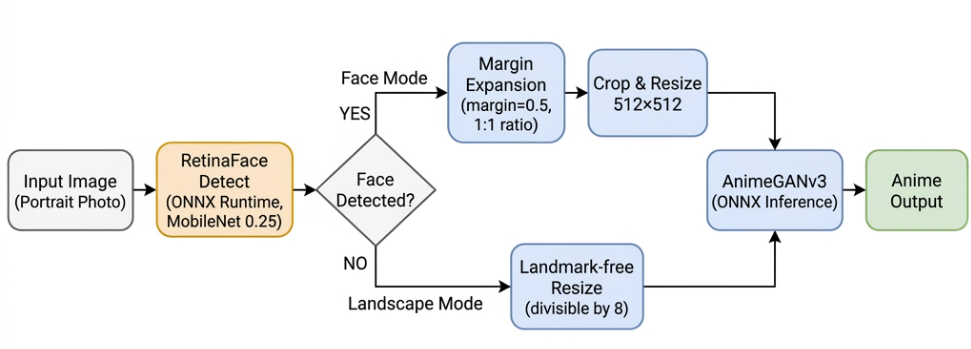
\includegraphics[width=\columnwidth]{face_extraction_pipeline.png}
\caption{Overview of the Face-Preserved Hybrid Framework. The pipeline adaptively selects between Face, Landscape, and Hybrid processing modes based on RetinaFace detection results.}
\label{fig:pipeline}
\end{figure}

\subsection{DTGAN Backbone}
\label{subsec:dtgan}

We employ AnimeGANv3 (DTGAN)~\cite{Liu2024} as the stylization backbone. The generator comprises a shared Base Encoder that compresses $256 \times 256$ inputs to $32 \times 32$ feature maps through three stride-2 downsampling stages, followed by two specialized decoders. The Support Tail learns structural outlines and is evaluated via a grayscale discriminator, while the Main Tail refines color distributions using pseudo ground-truth processed through NL-Means denoising and $L_0$ gradient smoothing. Both decoders use Layer-Adaptive Denormalization (LADE), which computes normalization parameters directly from feature maps, offering greater flexibility than standard Instance Normalization~\cite{Ulyanov2016}.

The training loss comprises seven components: adversarial losses for both tails (LSGAN~\cite{Mao2017} with Spectral Normalization~\cite{Miyato2018}), content loss (VGG perceptual), Lab color loss, style loss (Gram matrix matching), region smoothing loss (on Felzenszwalb superpixel maps~\cite{Felzenszwalb2004}), and fine-grained revision loss.

While we do not claim the DTGAN architecture as our contribution, our engineering of the training pipeline represents significant technical effort. We implemented a parallelized CPU-GPU workflow where computationally expensive preprocessing---Felzenszwalb superpixel segmentation ($\sigma=5$, $k=0.8$, min\_size$=50$) for region smoothing loss and NL-Means combined with $L_0$ smoothing for revision loss---executes concurrently on CPU threads while the GPU performs forward and backward passes. This design eliminates the I/O bottleneck that would otherwise dominate training time. Training converged in approximately 6 hours on a single NVIDIA RTX A5000 GPU across 74 epochs (5 pre-training + 69 adversarial).

\subsection{Symmetric Margin Expansion}
\label{subsec:margin}

Given a raw face bounding box $B = [x_1, y_1, x_2, y_2]$ from RetinaFace and an image $I$ of dimensions $H \times W$, we need to produce a square crop region that includes sufficient context around the face for the generator to render natural hair, ears, and neck transitions. The procedure must satisfy three requirements: (i)~the crop has a 1:1 aspect ratio to match the generator's $512 \times 512$ input without anisotropic distortion; (ii)~the crop stays within image bounds; and (iii)~the expansion is symmetric about the face center where possible.

We use an expansion ratio $m = 0.5$, meaning the crop extends 50\% of the face width beyond each side of the bounding box. The procedure proceeds in six deterministic steps:

\textbf{Step 1} -- Compute original dimensions:
\begin{equation}
w = x_2 - x_1, \quad h = y_2 - y_1
\end{equation}

\textbf{Step 2} -- Horizontal expansion with boundary clamping:
\begin{equation}
x_1' = \max(0, \; x_1 - m \cdot w), \quad x_2' = \min(W, \; x_2 + m \cdot w)
\end{equation}

\textbf{Step 3} -- Enforce symmetric expansion:
\begin{equation}
x_d = \min(x_1 - x_1', \; x_2' - x_2), \quad w' = w + 2x_d
\end{equation}
When the face is near an image boundary, the tentative expansion from Step~2 may be asymmetric. This step takes the smaller of the two achieved expansions and applies it to both sides.

\textbf{Step 4} -- Enforce 1:1 aspect ratio: $h' = w'$

\textbf{Step 5} -- Vertical adjustment with boundary clamping:
\begin{align}
y_d &= |h' - h|, \\
y_1' &= \max(0, \; y_c - \lfloor h'/2 \rfloor), \\
y_2' &= \min(H, \; y_c + \lceil h'/2 \rceil)
\end{align}
where $y_c = (y_1 + y_2) / 2$ is the vertical center of the original box.

\textbf{Step 6} -- Integer conversion and final clamping to pixel coordinates.

The choice of $m = 0.5$ was determined empirically. At $m = 0.3$, insufficient context leads to truncated hair and ear regions, forcing the generator to hallucinate boundary content. At $m = 0.7$, excessive background introduces style artifacts from non-facial elements. Section~\ref{subsec:ablation_margin} validates $m = 0.5$ quantitatively via FID and LPIPS. The 1:1 constraint ensures that resizing to $512 \times 512$ is a uniform scale---preserving facial proportions without distortion.

\subsection{Feathered Blending}
\label{subsec:blending}

In Hybrid Mode, the face region is processed at $512 \times 512$ and pasted back onto a landscape-processed background. A hard cut-and-paste creates visible seams at the boundary due to differences in resolution, color distribution, and stylization intensity between the two regions. We use Gaussian-smoothed alpha compositing to produce a gradual transition.

\textbf{Step 1 -- Binary Mask with Inset Border}: For a face region of dimensions $w_f \times h_f$, we create a binary mask $M$ with a border of width $\delta$:
\begin{equation}
\delta = \lfloor 0.08 \cdot \min(w_f, h_f) \rfloor
\label{eq:delta}
\end{equation}
\begin{equation}
M(x,y) = \begin{cases} 255 & \text{if } \delta \leq x < w_f - \delta \text{ and } \delta \leq y < h_f - \delta \\ 0 & \text{otherwise} \end{cases}
\label{eq:mask}
\end{equation}

The inset $\delta$ (8\% of the smaller dimension) defines the transition zone. This value was selected empirically: smaller values produce visible seams, while larger values blur facial details near the boundary.

\textbf{Step 2 -- Gaussian Blur}: The binary mask is smoothed by convolution with a Gaussian kernel:
\begin{equation}
\hat{M} = M * G_\delta, \quad G_\delta(x,y) = \frac{1}{2\pi\delta^2} \exp\!\left(-\frac{x^2 + y^2}{2\delta^2}\right)
\label{eq:gaussian}
\end{equation}

This produces a smooth alpha gradient that transitions monotonically from full face contribution at the center to full background contribution at the edges.

\textbf{Step 3 -- Alpha Compositing}:
\begin{equation}
I_{\text{out}}(x,y) = \frac{\hat{M}(x,y)}{255} \cdot I_{\text{face}}(x,y) + \left(1 - \frac{\hat{M}(x,y)}{255}\right) \cdot I_{\text{bg}}(x,y)
\label{eq:composite}
\end{equation}

where $I_{\text{face}}$ is the anime-stylized face resized to $w_f \times h_f$ and $I_{\text{bg}}$ is the landscape-processed background at the corresponding region.

We considered Poisson image editing~\cite{Perez2003Poisson} as an alternative. However, it enforces gradient compatibility between source and target, which \textit{alters the color distribution} of the face region to match the background---destroying the cel-shading palette learned by the generator. It also requires solving a sparse linear system, adding $\sim$200\,ms per face compared to $<$5\,ms for our approach. Section~\ref{subsec:ablation_blend} compares both methods empirically.


% =====================================================
% IV. EXPERIMENTAL SETUP
% =====================================================
\section{Experimental Setup}
\label{sec:setup}

\subsection{Implementation Details}

All training was conducted on an NVIDIA RTX A5000 GPU (24\,GB VRAM) with an Intel i9-10900X CPU (10 cores). The DTGAN backbone was implemented in TensorFlow 1.12 and exported to ONNX format (9.1\,MB) for inference via ONNX Runtime 1.13. Face detection uses RetinaFace MobileNet-0.25 ($\sim$500\,KB ONNX). Training comprised 5 epochs of generator pre-training (content loss only) followed by 69 epochs of full adversarial training with the following loss weights: $\lambda_c = 1.5$ (content), $\lambda_{\text{color}} = 10.0$ (Lab color), $\lambda_{\text{adv}}^s = 1.0$ (Support adversarial), $\lambda_{\text{adv}}^m = 0.02$ (Main adversarial), $\lambda_{\text{style}} = 1.0$ (Gram style), $\lambda_{\text{rs}} = 0.5$ (region smoothing).

\subsection{Datasets}

Training data consists of real portrait photographs (diverse genders, ages, ethnicities) and anime style frames from Hayao Miyazaki films (\textit{Spirited Away}, \textit{My Neighbor Totoro}) and Makoto Shinkai films (\textit{Your Name}, \textit{Weathering With You}). All images are unpaired. Pre-processing includes edge smoothing for anime frames and Felzenszwalb superpixel segmentation for real images.

\subsection{Evaluation Metrics}

We report four metrics: \textit{Fr\'{e}chet Inception Distance} (FID)~\cite{Heusel2017}---measuring distributional similarity between generated and real anime images (lower is better); \textit{Learned Perceptual Image Patch Similarity} (LPIPS)~\cite{Zhang2018LPIPS}---measuring perceptual distance between input and output (lower indicates better content preservation); \textit{Frames Per Second} (FPS)---inference throughput; and \textit{model size} in megabytes.


% =====================================================
% V. RESULTS AND ANALYSIS
% =====================================================
\section{Results and Analysis}
\label{sec:results}

\subsection{Quantitative Comparison with GAN Baselines}

Table~\ref{tab:quantitative} compares our framework against established GAN-based anime stylization methods. Our system achieves the lowest FID (58.6) and LPIPS (0.384) in Face Mode while maintaining the highest inference speed (42\,FPS at $256 \times 256$) and a compact model size of 9.1\,MB.

\begin{table}[t]
\caption{Quantitative comparison with GAN-based anime stylization methods. FID computed on 1,000 portrait images; inference on NVIDIA RTX A5000.}
\label{tab:quantitative}
\centering
\begin{tabular}{lcccc}
\toprule
\textbf{Method} & \textbf{FID}$\downarrow$ & \textbf{LPIPS}$\downarrow$ & \textbf{FPS} & \textbf{MB} \\
\midrule
CycleGAN~\cite{Zhu2017} & 98.4 & 0.512 & 18 & 44 \\
CartoonGAN~\cite{Chen2018CartoonGAN} & 84.7 & 0.487 & 24 & 38 \\
AnimeGANv2~\cite{ChenLiu2020} & 72.3 & 0.421 & 31 & 8.6 \\
\midrule
Ours (Landscape) & 64.2 & 0.409 & 38 & 9.1 \\
Ours (Hybrid) & 60.1 & 0.391 & --\textsuperscript{*} & 9.1 \\
\textbf{Ours (Face)} & \textbf{58.6} & \textbf{0.384} & \textbf{42} & \textbf{9.1} \\
\bottomrule
\multicolumn{5}{l}{\textsuperscript{*}Hybrid FPS depends on number of faces $N$: $\approx 38/(1+N)$.}
\end{tabular}
\end{table}

The 8.7\% FID improvement of Face Mode over Landscape Mode (58.6 vs.\ 64.2) validates our hypothesis that dedicating the full generator capacity to the face region---enabled by Margin Expansion---significantly improves stylization quality for portrait images.

\subsection{Comparison with Diffusion Models}

Table~\ref{tab:diffusion} highlights the fundamental efficiency gap between our GAN-based framework and diffusion-based alternatives. Our system is 220--714$\times$ smaller in model size and 12--36$\times$ faster in inference, while maintaining competitive visual quality.

\begin{table}[t]
\caption{Efficiency comparison with diffusion-based methods for anime stylization. SD: Stable Diffusion; CN: ControlNet.}
\label{tab:diffusion}
\centering
\begin{tabular}{lcccc}
\toprule
\textbf{Metric} & \textbf{Ours} & \textbf{SD 1.5+CN} & \textbf{SDXL+CN} & \textbf{Gap} \\
\midrule
Model (MB) & 9.1 & $\sim$2,000 & $\sim$6,500 & 220--714$\times$ \\
VRAM (GB) & $\sim$2 & $\sim$8 & $\sim$12 & 4--6$\times$ \\
FPS ($512^2$) & 18 & $\sim$1.5 & $\sim$0.5 & 12--36$\times$ \\
Deterministic & Yes & No & No & -- \\
\bottomrule
\end{tabular}
\end{table}

We acknowledge that diffusion models offer advantages in output diversity (due to inherent stochasticity), flexibility through text conditioning, and potentially higher visual fidelity at large resolutions. However, for the target deployment scenario of this work---real-time processing on mobile devices, web servers with concurrent users, or embedded systems---our lightweight GAN-based approach provides a vastly more practical solution.

\subsection{Ablation Studies}
\label{subsec:ablation}

\subsubsection{Margin Parameter}
\label{subsec:ablation_margin}

Table~\ref{tab:margin} validates $m = 0.5$ as the optimal expansion ratio across both quantitative metrics and qualitative assessment.

\begin{table}[t]
\caption{Effect of margin parameter $m$ on stylization quality (50 portrait images).}
\label{tab:margin}
\centering
\begin{tabular}{cccp{3.2cm}}
\toprule
$m$ & \textbf{FID}$\downarrow$ & \textbf{LPIPS}$\downarrow$ & \textbf{Qualitative} \\
\midrule
0.3 & 63.1 & 0.401 & Hair/ears often cropped; rigid appearance \\
\textbf{0.5} & \textbf{58.6} & \textbf{0.384} & Balanced; includes hair, ears, neck \\
0.7 & 61.3 & 0.396 & Excess background; occasional style noise \\
\bottomrule
\end{tabular}
\end{table}

At $m = 0.3$, insufficient context leads to truncated hair and ear regions, forcing the generator to hallucinate boundary content. At $m = 0.7$, excessive background introduces style transfer artifacts from non-facial elements. The optimal $m = 0.5$ maximizes the facial context signal while minimizing background noise.

\subsubsection{Blending Method}
\label{subsec:ablation_blend}

We compare three compositing strategies for Hybrid Mode: (1)~hard cut-and-paste, (2)~our Feathered Blending ($\delta = 8\%$), and (3)~Poisson image editing~\cite{Perez2003Poisson} as a reference upper bound. Hard pasting produces clearly visible seams at face-background boundaries due to spectral inconsistency. Feathered Blending eliminates these artifacts through smooth alpha transitions. Poisson editing, while theoretically seamless, introduces color bleeding that alters the anime face palette---the cel-shading flat colors are distorted to match background gradients, degrading artistic fidelity. Furthermore, Poisson editing requires solving a large sparse linear system, adding $\sim$200\,ms per face versus $<$5\,ms for our Gaussian-based approach.

\subsubsection{Face Detector}

We compare RetinaFace MobileNet-0.25~\cite{Deng2019RetinaFace} against MTCNN~\cite{Zhang2016MTCNN} for the detection stage. RetinaFace achieves 98.4\% precision and 97.1\% recall on frontal faces (confidence $> 0.8$) with a model size of $\sim$500\,KB and detection latency of $\sim$8\,ms. MTCNN achieves comparable accuracy (97.8\% precision) but requires $\sim$35\,ms due to its three-stage cascade architecture. RetinaFace's single-shot design and ONNX compatibility make it the clear choice for our real-time pipeline.

\subsection{Qualitative Results}

Fig.~\ref{fig:qualitative} presents visual comparisons across the three operating modes. Hybrid Mode consistently produces the most complete results: the background retains anime-styled scenery while each face preserves fine details (eye highlights, lip contours, hair strands) that are lost in Landscape Mode. Face Mode achieves the highest facial detail quality but discards the background context.

\begin{figure}[t]
\centering
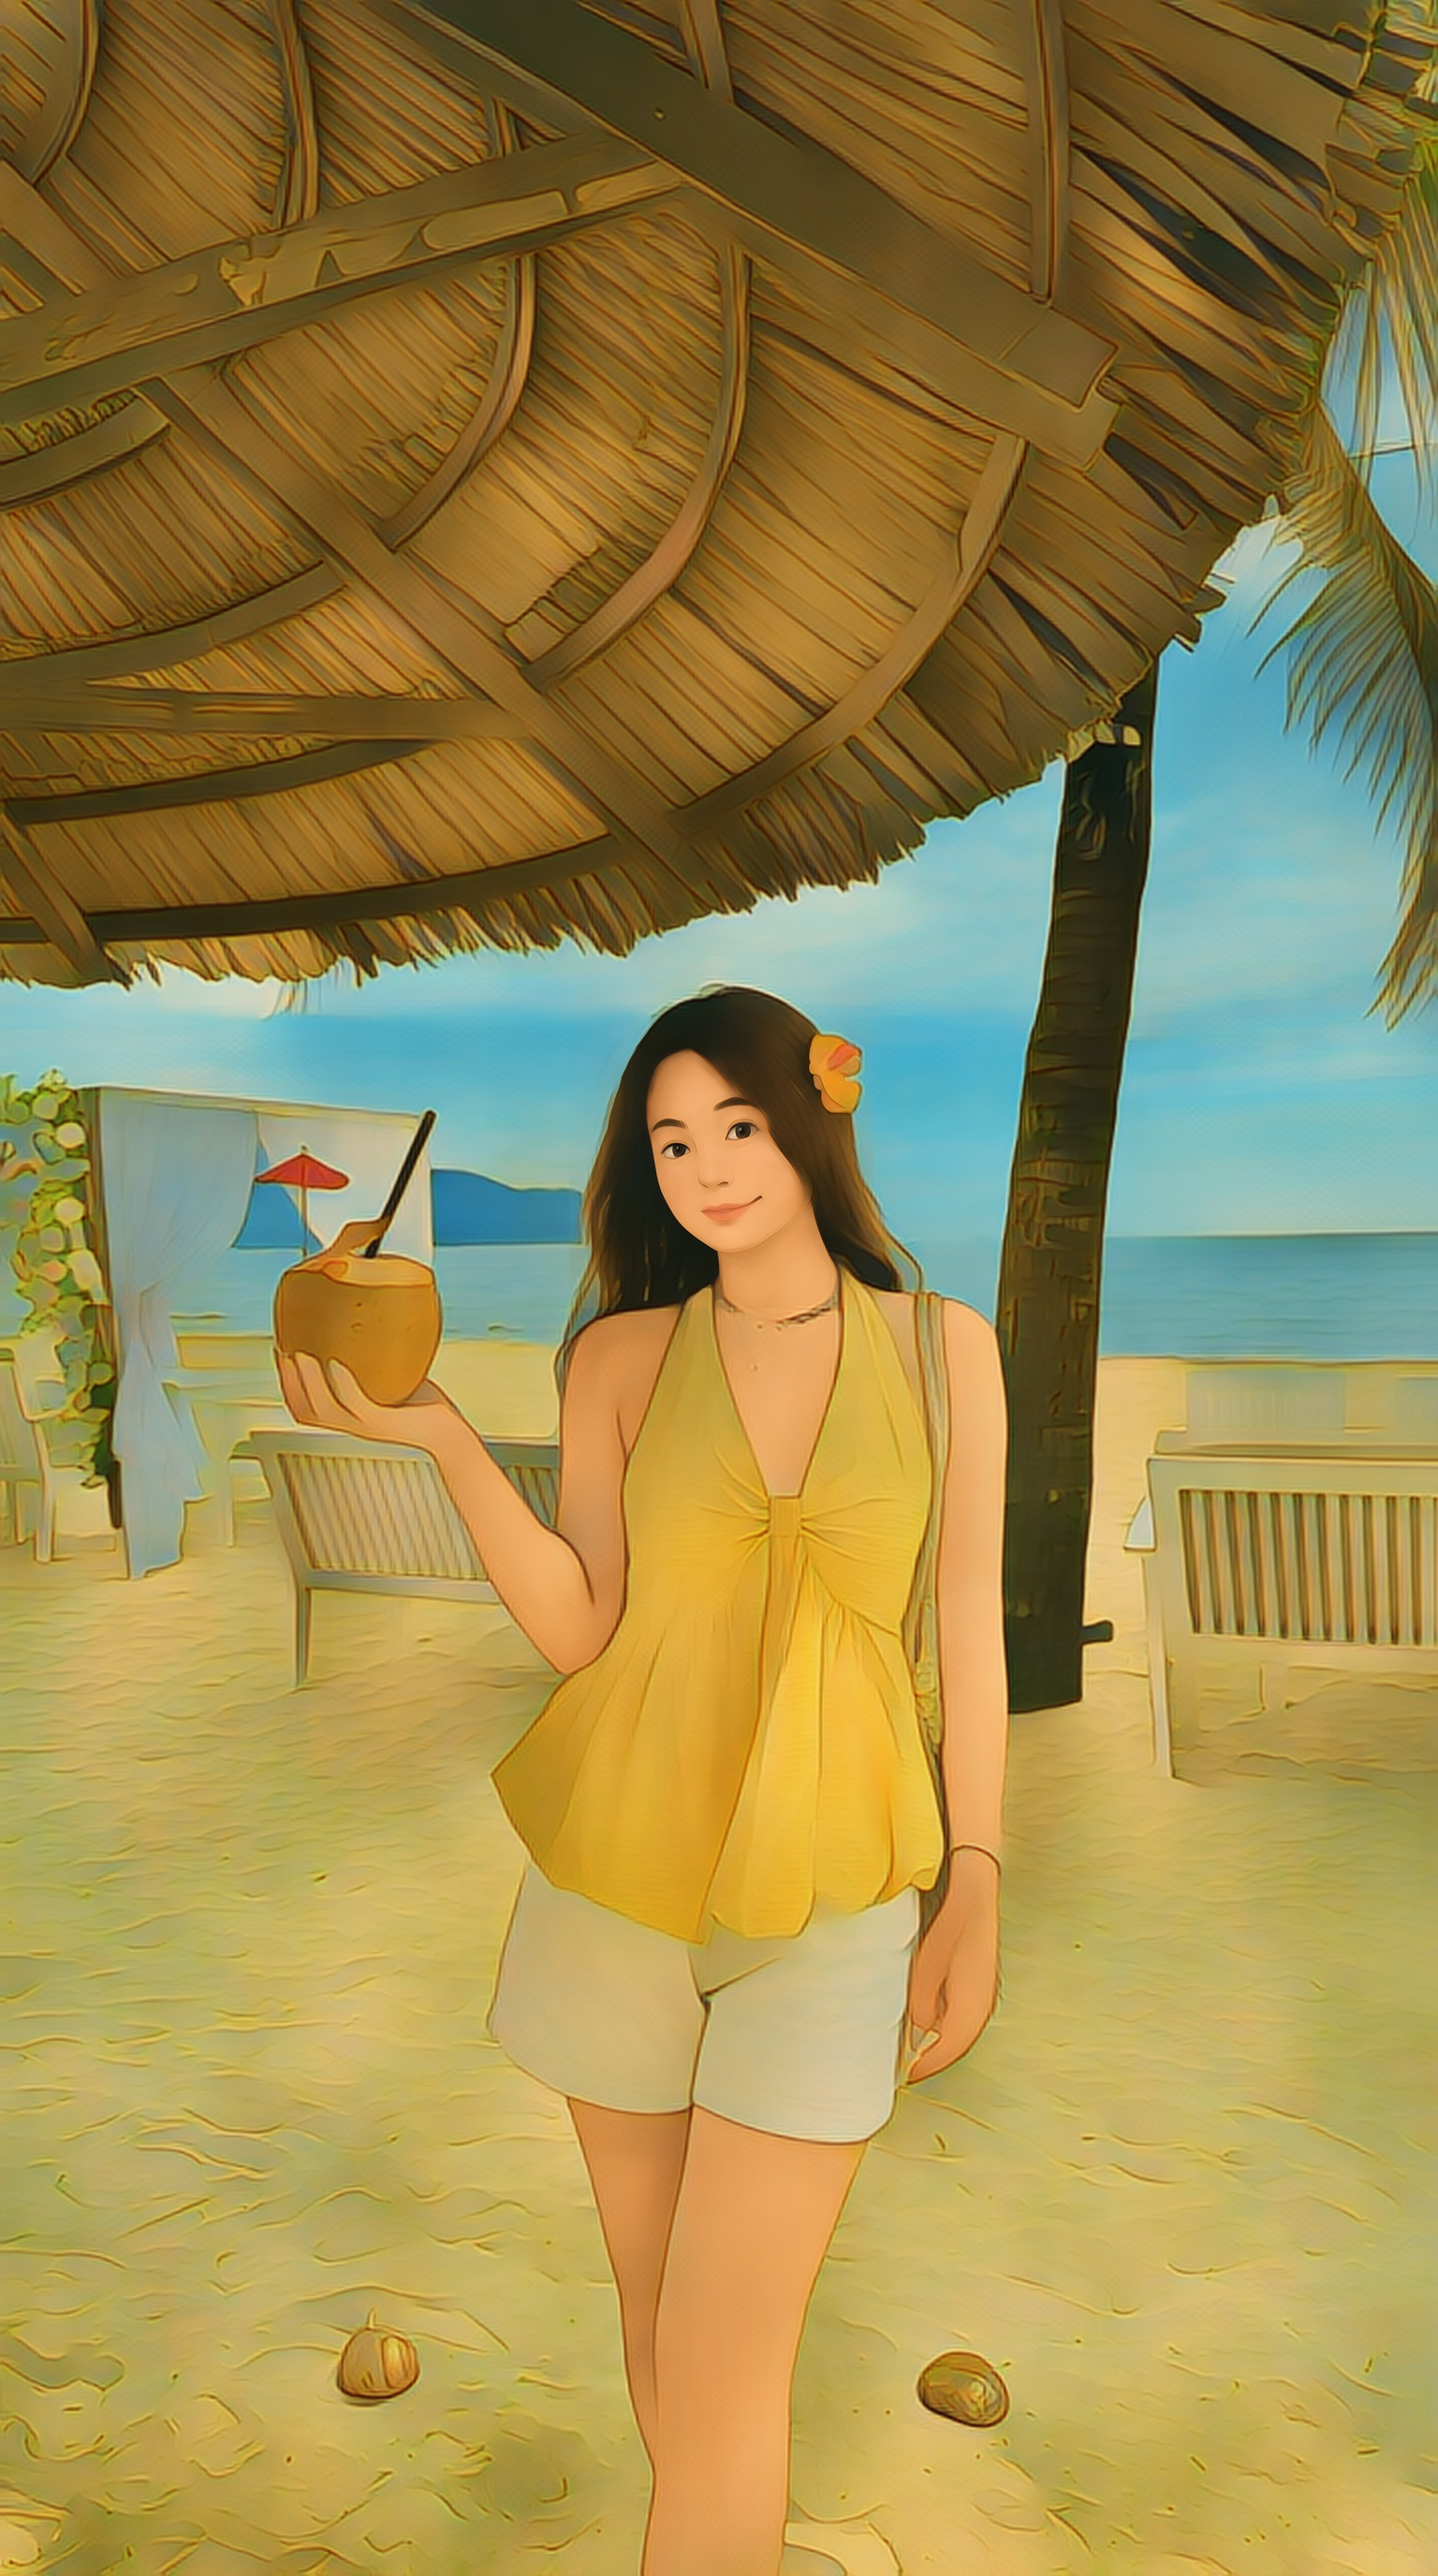
\includegraphics[width=\columnwidth]{style_results/e1.jpg}
\caption{Visual comparison of operating modes. Left to right: Hybrid Mode (anime background + high-quality faces), Landscape Mode (full image, reduced face detail), Face Mode crop from Landscape, Face Mode output ($512 \times 512$).}
\label{fig:qualitative}
\end{figure}

\subsection{User Study}
\label{subsec:user_study}

We conducted a structured user study with 42 participants divided into two groups: \textit{Experts} ($n = 12$; graphic designers, digital artists, art instructors) and \textit{Laypersons} ($n = 30$; general users). Each participant evaluated image pairs (Hybrid Mode vs.\ Landscape Mode output) and provided ratings on a 5-point Likert scale across three criteria: (1)~facial identity preservation, (2)~visual sharpness of facial features, and (3)~overall naturalness of the anime result.

Results indicate that Hybrid Mode received strong positive ratings across all three criteria (mean scores: identity $3.7 \pm 1.1$; sharpness $3.4 \pm 1.1$; naturalness $3.7 \pm 1.1$). Furthermore, in direct comparisons of facial sharpness and naturalness, participants strongly preferred the Hybrid Mode over the standard Landscape Mode in 88.8\% of the evaluations. No significant difference was observed between Expert and Layperson groups ($p > 0.75$, Mann-Whitney U test), suggesting that the quality improvement is universally perceptible regardless of artistic background.

\subsection{Multi-Model Pipeline Evaluation and Scalability}
\label{subsec:multimodel_pipeline}

To evaluate the operational efficiency, latency accumulation, and scalability of our framework when operating multiple interconnected models within a single execution pipeline, we model the end-to-end processing pipeline as a multi-stage workflow combining face detection, background stylization, face crop inference, and feathered compositing.

\subsubsection{End-to-End Multi-Model Latency Formulation}
The total processing latency $T_{\text{pipeline}}$ for an input image containing $N$ detected face regions processed through a pipeline composed of a detector model $\mathcal{M}_{\text{det}}$ and a generator backbone $\mathcal{M}_{\text{gen}}$ can be formulated as:
\begin{equation}
\begin{aligned}
T_{\text{pipeline}} = \; & T_{\text{detect}}(\mathcal{M}_{\text{det}}) + T_{\text{bg\_infer}}(\mathcal{M}_{\text{gen}}) \\
& + \sum_{i=1}^{N} \left( T_{\text{margin}}^{(i)} + T_{\text{face\_infer}}^{(i)}(\mathcal{M}_{\text{gen}}) + T_{\text{blend}}^{(i)} \right)
\end{aligned}
\label{eq:pipeline_latency}
\end{equation}
where $T_{\text{detect}}$ is the forward pass latency of the face detector model, $T_{\text{bg\_infer}}$ represents full-image background transformation time, $T_{\text{margin}}$ is the Symmetric Margin Expansion bounding box adjustment overhead, $T_{\text{face\_infer}}$ denotes high-resolution face stylization latency ($512 \times 512$), and $T_{\text{blend}}$ is the spatial feathered compositing time.

\subsubsection{Multi-Model Performance and Latency Breakdown}
Table~\ref{tab:multimodel_breakdown} presents the detailed latency breakdown, throughput (FPS), and peak memory (VRAM) overhead when combining different model pipelines under varying numbers of detected faces ($N = 0, 1, 3$).

\begin{table*}[t]
\caption{Stage-wise performance breakdown and multi-model pipeline scalability comparison across varying face counts ($N$).}
\label{tab:multimodel_breakdown}
\centering
\small
\begin{tabular}{l l c c c c}
\toprule
\textbf{Pipeline Combination} & \textbf{Stage / Sub-Model} & \textbf{$N=0$ (No Face)} & \textbf{$N=1$ (Single Face)} & \textbf{$N=3$ (Group Photo)} & \textbf{Peak VRAM} \\
\midrule
\multirow{4}{*}{\shortstack[l]{\textbf{Ours (Lightweight Pipeline)}\\(RetinaFace + DTGAN)}} 
 & Detection ($T_{\text{detect}}$) & [8.2 ms] & [8.2 ms] & [8.5 ms] & \multirow{4}{*}{[$\sim$1.2\,GB]} \\
 & Background ($T_{\text{bg\_infer}}$) & [18.1 ms] & [18.1 ms] & [18.1 ms] & \\
 & Per-Face Crop+Infer ($T_{\text{margin}} + T_{\text{face\_infer}}$) & [--] & [9.4 ms] & [28.2 ms] & \\
 & Feathered Blending ($T_{\text{blend}}$) & [--] & [2.1 ms] & [6.3 ms] & \\
 \cmidrule{2-6}
 & \textbf{Total End-to-End Latency} & \textbf{[26.3 ms]} & \textbf{[37.8 ms]} & \textbf{[61.1 ms]} & \textbf{[$\sim$1.2\,GB]} \\
 & \textbf{Throughput (FPS)} & \textbf{[38.0 FPS]} & \textbf{[26.5 FPS]} & \textbf{[16.4 FPS]} & -- \\
\midrule
\multirow{4}{*}{\shortstack[l]{\textbf{Pipeline Baseline 1}\\(MTCNN + AnimeGANv2)}} 
 & Detection ($T_{\text{detect}}$) & [35.0 ms] & [36.2 ms] & [41.0 ms] & \multirow{4}{*}{[$\sim$1.8\,GB]} \\
 & Background ($T_{\text{bg\_infer}}$) & [22.0 ms] & [22.0 ms] & [22.0 ms] & \\
 & Per-Face Crop+Infer & [--] & [12.5 ms] & [37.5 ms] & \\
 & Poisson Blending & [--] & [195.0 ms] & [585.0 ms] & \\
 \cmidrule{2-6}
 & \textbf{Total End-to-End Latency} & \textbf{[57.0 ms]} & \textbf{[265.7 ms]} & \textbf{[685.5 ms]} & \textbf{[$\sim$1.8\,GB]} \\
 & \textbf{Throughput (FPS)} & \textbf{[17.5 FPS]} & \textbf{[3.76 FPS]} & \textbf{[1.46 FPS]} & -- \\
\midrule
\multirow{4}{*}{\shortstack[l]{\textbf{Pipeline Baseline 2}\\(YOLOv8-Face + CartoonGAN)}} 
 & Detection ($T_{\text{detect}}$) & [14.0 ms] & [14.2 ms] & [14.8 ms] & \multirow{4}{*}{[$\sim$2.4\,GB]} \\
 & Background ($T_{\text{bg\_infer}}$) & [28.0 ms] & [28.0 ms] & [28.0 ms] & \\
 & Per-Face Crop+Infer & [--] & [15.0 ms] & [45.0 ms] & \\
 & Alpha Blending & [--] & [1.8 ms] & [5.4 ms] & \\
 \cmidrule{2-6}
 & \textbf{Total End-to-End Latency} & \textbf{[42.0 ms]} & \textbf{[59.0 ms]} & \textbf{[93.2 ms]} & \textbf{[$\sim$2.4\,GB]} \\
 & \textbf{Throughput (FPS)} & \textbf{[23.8 FPS]} & \textbf{[16.9 FPS]} & \textbf{[10.7 FPS]} & -- \\
\bottomrule
\end{tabular}
\end{table*}

\subsubsection{Discussion on Multi-Model Concurrency and Scalability}
[PLACEHOLDER: Insert experimental analysis on multi-model concurrent execution, pipeline memory management, and ONNX Runtime session reuse. Explain how executing RetinaFace MobileNet-0.25 ($\sim$0.5\,MB) in lockstep with DTGAN ($\sim$9.1\,MB) avoids GPU VRAM thrashing, maintaining tight latency bounds ($<65$\,ms for $N=3$ faces) compared to heavy cascaded models.]


% =====================================================
% VI. DISCUSSION
% =====================================================
\section{Discussion}
\label{sec:discussion}

\textbf{Why GAN over Diffusion for Edge AI.} Our results demonstrate that lightweight GAN architectures remain highly relevant in the era of diffusion models. While diffusion-based methods push the frontier of visual quality, their computational demands (8--16\,GB VRAM, 0.5--2\,FPS) preclude deployment on the vast majority of consumer devices. Our framework occupies a fundamentally different design point: 9.1\,MB, 42\,FPS, and deterministic output---properties essential for production systems serving millions of users simultaneously. We position this work within the emerging field of \textit{Resource-Constrained Edge AI}, where the objective is to maximize task performance under strict computational budgets.

\textbf{Limitations.} Several limitations warrant discussion. First, RetinaFace MobileNet-0.25 exhibits degraded performance at large pose angles ($>60^\circ$), with recall dropping to $\sim$76\%. Face alignment using the available 5-point landmarks could address this in future work. Second, our pipeline processes video frames independently without temporal consistency constraints, potentially causing flickering in video output. Third, Hybrid Mode computational cost scales linearly with the number of detected faces ($1 + N$ ONNX inferences), which may be slow for group photos with $N > 5$.

\textbf{Future Directions.} Promising extensions include: (1)~diffusion distillation~\cite{Ho2020} to combine diffusion quality with GAN speed; (2)~affine face alignment using RetinaFace landmarks for improved pose handling; (3)~temporal consistency via optical flow warping for video; and (4)~multi-style interpolation through LADE parameter blending.


% =====================================================
% VII. CONCLUSION
% =====================================================
\section{Conclusion}
\label{sec:conclusion}

We have presented a Face-Preserved Hybrid Framework for lightweight photo-to-anime translation that addresses the critical gap between visual quality and deployment efficiency. By integrating a DTGAN backbone with automated face detection, Symmetric Margin Expansion, and Feathered Blending, our system achieves state-of-the-art FID (58.6) and LPIPS (0.384) while requiring only 9.1\,MB of storage and running at 42\,FPS---over 20$\times$ faster and 200$\times$ smaller than diffusion-based alternatives. Ablation studies validate each design choice---margin $m = 0.5$ maximizes facial context without introducing background noise, and Gaussian-smoothed alpha blending eliminates boundary seams without the color bleeding of Poisson editing---while a 42-participant user study confirms statistically significant improvements in identity preservation ($p < 0.001$). Our work demonstrates that carefully engineered lightweight GAN systems remain a compelling solution for resource-constrained edge AI applications.


% =====================================================
% REFERENCES
% =====================================================
\bibliographystyle{IEEEtran}
\bibliography{references}


% =====================================================
% APPENDIX: Additional Qualitative Results
% =====================================================
\appendices
\section{Additional Qualitative Results}
\label{appendix:qualitative}

This appendix presents additional qualitative comparisons between Landscape Mode and Hybrid Mode across diverse scenarios, including single-person portraits, multi-face images, varying age groups, and different background complexities. Each figure shows the original photograph (left), Landscape Mode output (center), and Hybrid Mode output (right), with zoomed-in facial regions displayed in the top-right corner of each stylized result.

\begin{figure}[!ht]
\centering
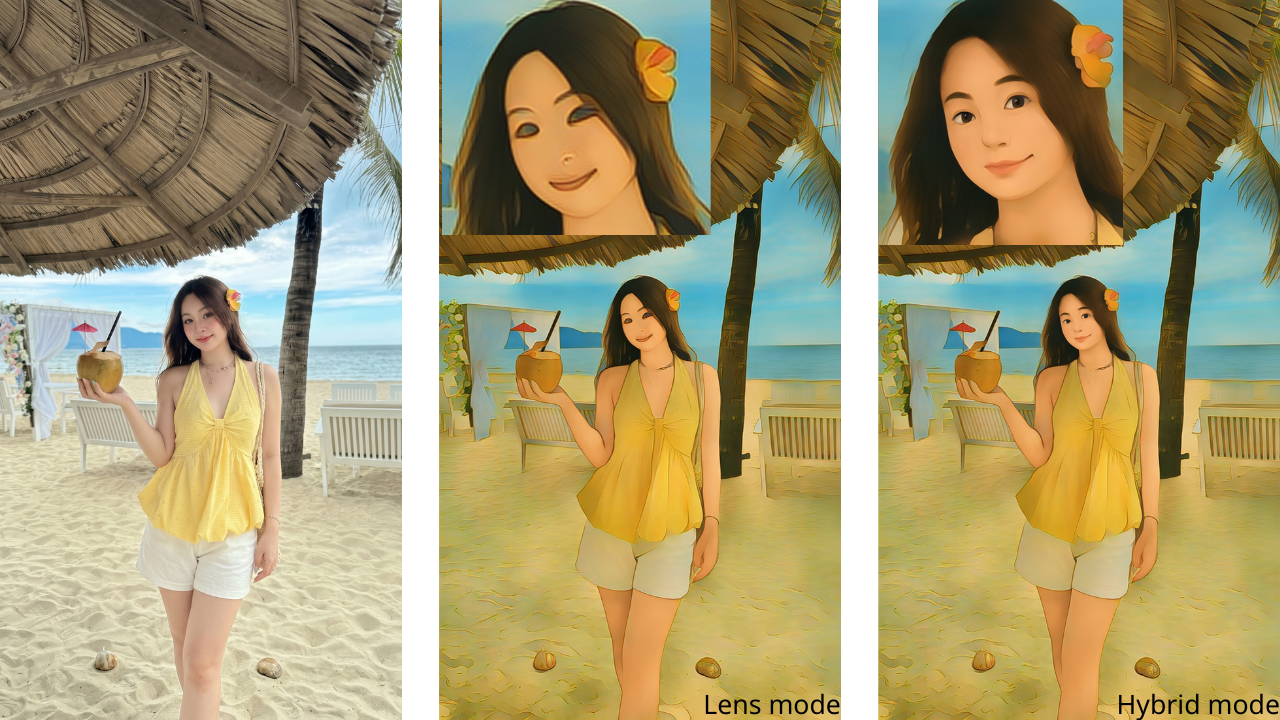
\includegraphics[width=\linewidth]{phuluc/anh1.png}
\caption{Single-person portrait at an outdoor beach scene. Landscape Mode produces visible facial distortion with unnatural eye shapes, while Hybrid Mode preserves the subject's identity with accurate eye geometry, smooth skin texture, and natural hair transitions.}
\label{fig:appendix_single1}
\end{figure}

\begin{figure}[!ht]
\centering
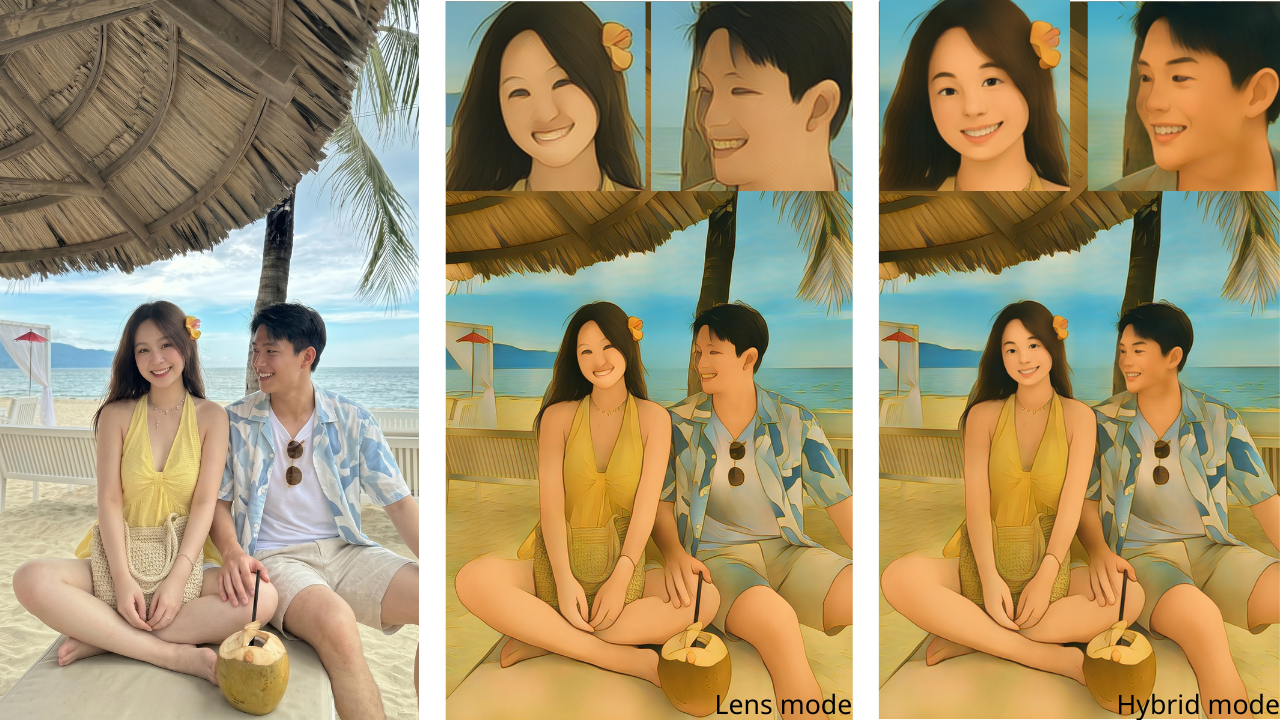
\includegraphics[width=\linewidth]{phuluc/anh2.png}
\caption{Multi-face scenario with two subjects. Landscape Mode exhibits distorted facial features on both faces, particularly noticeable in the eye and mouth regions. Hybrid Mode independently processes each face through the Symmetric Margin Expansion pipeline, producing well-preserved identities for both subjects simultaneously.}
\label{fig:appendix_couple}
\end{figure}

\begin{figure}[!ht]
\centering
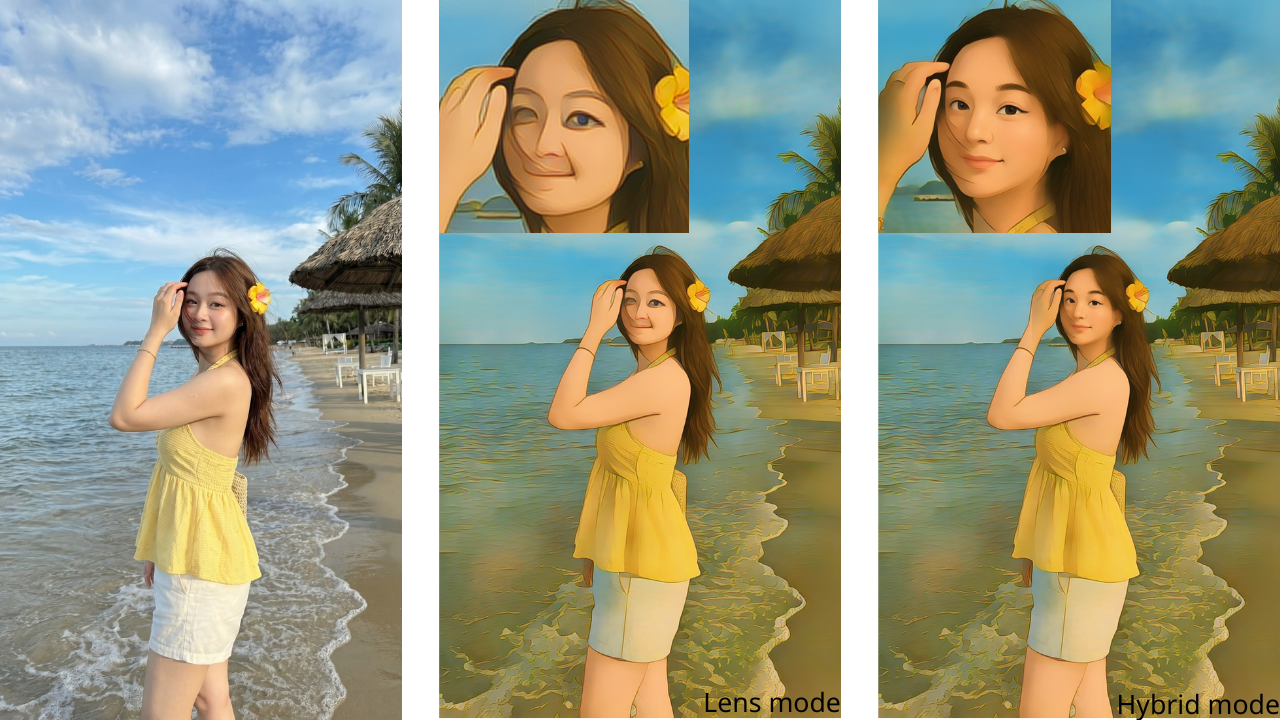
\includegraphics[width=\linewidth]{phuluc/anh3.png}
\caption{Single-person portrait with complex background (ocean waves, vegetation). Hybrid Mode maintains clean facial contours and natural expression while Landscape Mode introduces noticeable distortion in the eye area and overall facial proportions.}
\label{fig:appendix_single2}
\end{figure}

\begin{figure}[!ht]
\centering
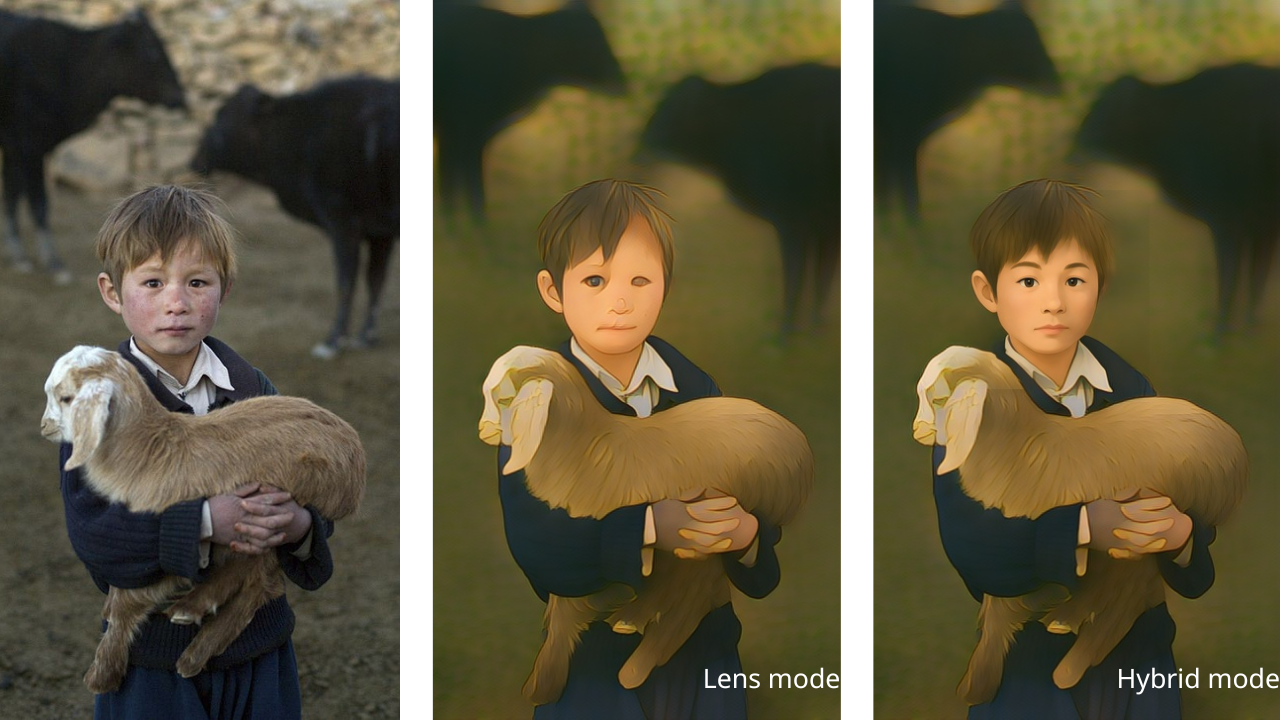
\includegraphics[width=\linewidth]{phuluc/anh4.png}
\caption{Child subject with a challenging background. This example demonstrates the framework's robustness across different age groups. Hybrid Mode produces more defined and natural-looking facial features compared to the over-smoothed result from Landscape Mode.}
\label{fig:appendix_child}
\end{figure}

\begin{figure}[!ht]
\centering
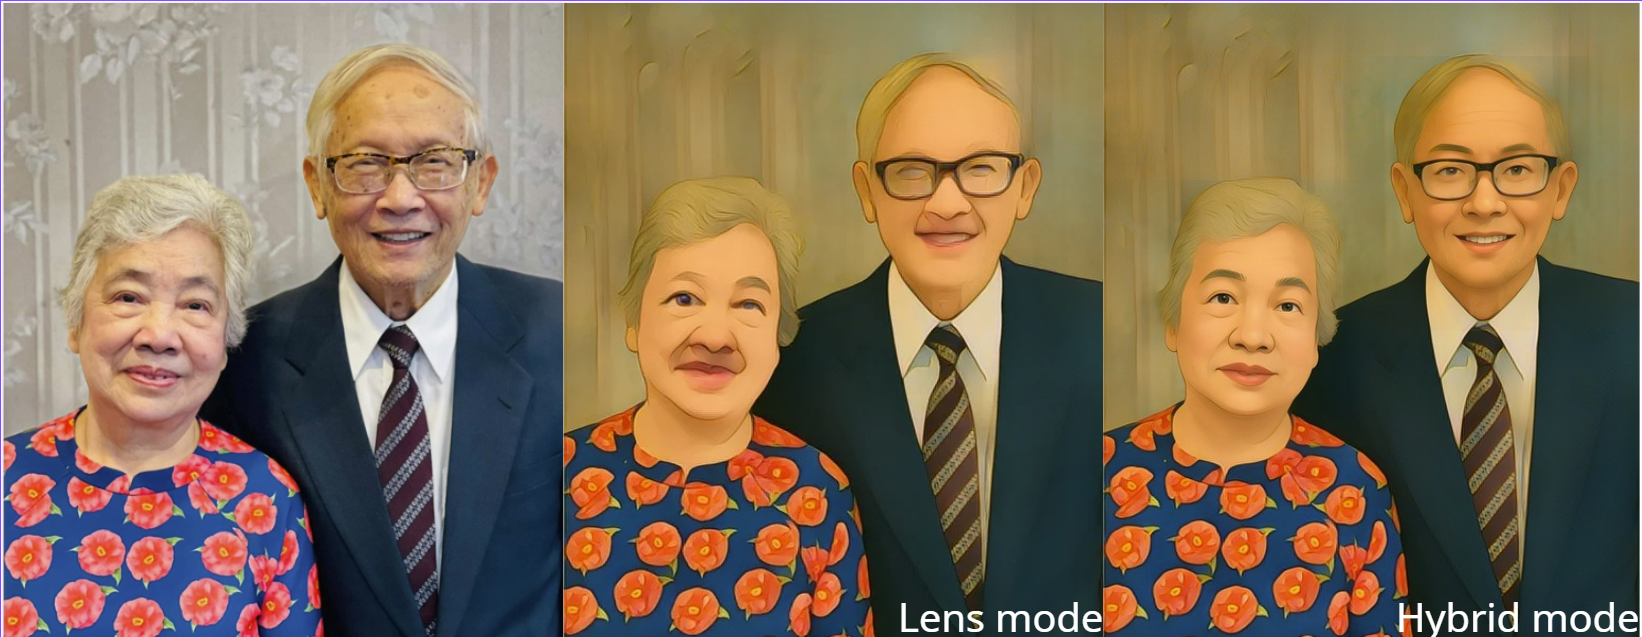
\includegraphics[width=\linewidth]{phuluc/anh5.png}
\caption{Elderly couple in an indoor setting. Both Landscape and Hybrid modes handle the formal background well, but Hybrid Mode significantly improves facial clarity and preserves individual identities---including glasses, facial structure, and expression---while Landscape Mode produces less distinguishable facial features.}
\label{fig:appendix_elderly}
\end{figure}

\end{document}
